\subsection{Comparative Experimental Evaluation of \ac{AMBC} \\
                 During Pitch-Only Motion in the Presence \\
                 of Unmodeled Thruster Dynamics}
\label{chUV_AMBC.sec.singleDOFAnalysisFailure}


This Section reports two experiments using \ac{AMBC} to control the
\ac{JHUROV}. In the first experiment parameter adaptation is unstable;
in the second experiment parameter adaptation is stable. In both
experiments the vehicle follows a pitch-only reference trajectory; the
mass, drag, and gravitational terms were initialized to parameters
previously identified to model vehicle performance (tabulated in
Tables \ref{chUV_AMBC.tb.quasistatic} and
\ref{chUV_AMBC.tb.dynParam}); and the gains used were $k_p=300$,
$k_d=100$ $\gamma_{m_i}=1000$, $\gamma_{d_i}=5000$,
$\gamma_{g}=\gamma_{b_1}=\gamma_{b_2}=0.5$ and $\gamma_{b_3}=10.0$.
In the first experiment, the pitch-only reference trajectory
oscillates about zero pitch.  In the second experiment, pitch-only
reference trajectory oscillates about a mean pitch of $5^\circ$ with
an amplitude of $3^\circ$.  The first experiment requires thrust
reversals to follow the specified reference trajectory, and the second
experiment does not require thrust reversals.

Figure \ref{chUV_AMBC.fig.stictionErrorWithThRev} plots the pitch,
angular velocity, thrust commands, and mass estimate derivative for
the experiment with thrust reversals.  In the thrust subplots the four
lines are plotted, the commanded and estimated thrusts are shown for
the two thrusters actuating vehicle pitch.  Note that the thrust is
estimated using a thruster's measured angular velocity as detailed in
Appendix \ref{appenJHUHTF.sec.hydrolab}.  Note that for both thrusters
as the commanded thrust crosses zero, the measured output remains zero
until the commanded thrust reaches 5 Newtons.  The buoyancy torque's
influence causes the pitch and y angular velocity to significantly
deviate from their respective reference trajectories.  From the
perspective of the \ac{AMBC} algorithm, these deviations from the
position and velocity reference trajectories are indistinguishable
from the deviations which would occur if the estimated pitch inertia
were too large, thus the parameter estimate update for this term,
$\dot{\hat{m}}_5$, has a large negative spike after each thrust
reversal. Over a multi-hour experiment this systematic error causes
pitch and roll mass estimates to adapt to physically unrealistic
negative values.

Figure \ref{chUV_AMBC.fig.stictionErrorWithoutThRev} plots the pitch,
angular velocity, thrust commands, and mass estimate derivative for
the experiment without thrust reversals.  Without thrust reversals,
the chain of events leading to a large negative spike in the pitch
mass update law are not present. The balanced parameter adaptation
seen in this third experiment leads to pitch mass convergence to a
physically realistic value.

%The conditions for this type of ___ also exist in the roll DOF, but not
%in the other DOF of x, y, z, Heading

\begin{center}
\begin{figure*}[htbp]
  \begin{center}
    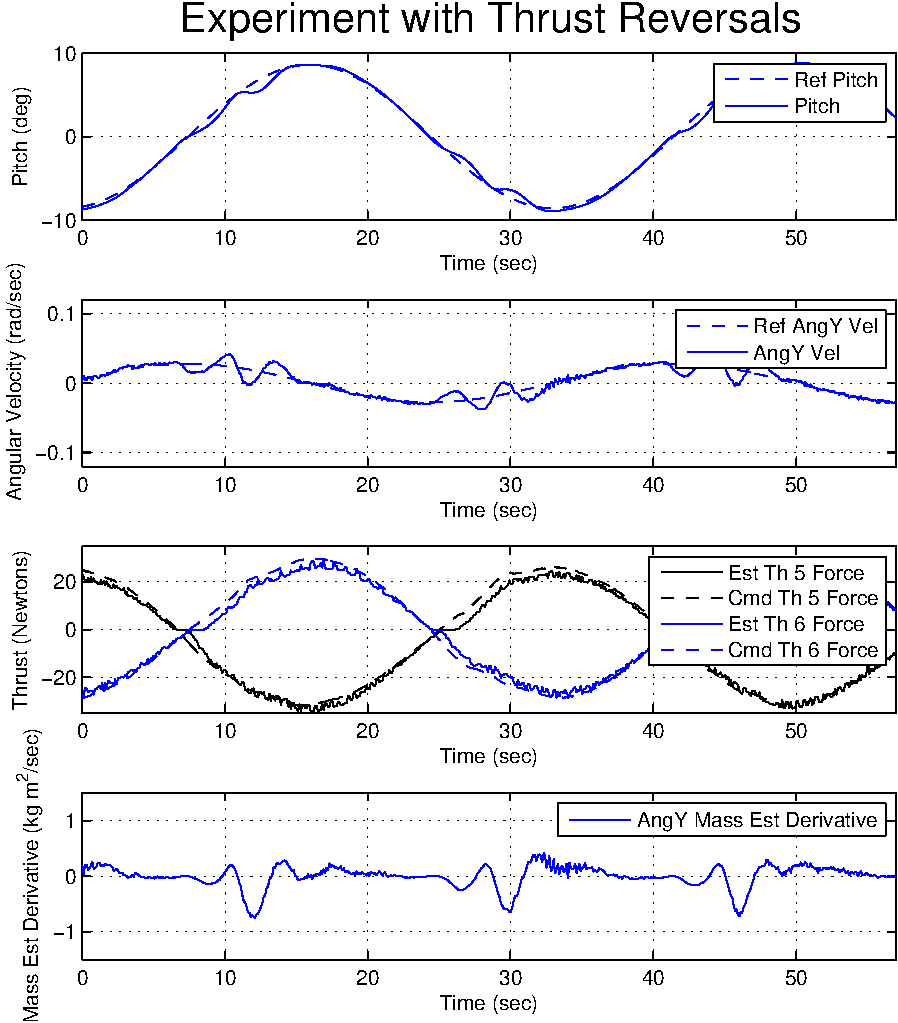
\includegraphics[width=150mm]{./chUV_AMBC/images/stictionErrorWithThrustReversals}
  \end{center}
  \caption{ 
%Data from two experiments where   For both
%    experiments an uncoupled model was assumed, initial parameter
%    estimates taken from the final values in Tables
%    \ref{chUV_AMBC.tb.quasistatic} and \ref{chUV_AMBC.tb.dynParam},
    Fifty five seconds of data from a experiment where \ac{AMBC} was used to
    follow a single \ac{DOF} reference trajectory in pitch.  Following
    the reference trajectory required thrust reversals. Thruster force
    was estimated using measured propeller angular velocity.  In the
    commanded/estimated thruster subplot, a short period of thruster
    stiction is seen at each thrust reversal.  The effects of thruster
    stiction are seen in both the pitch and angular velocity plots as
    deviations from each state's respective reference trajectory. In
    the pitch mass estimate derivative, the parameter update law is
    seen to have a large negative spike after each thrust reversal.}
  \label{chUV_AMBC.fig.stictionErrorWithThRev}
\end{figure*}
\end{center}

\begin{center}
\begin{figure*}[htbp]
  \begin{center}
    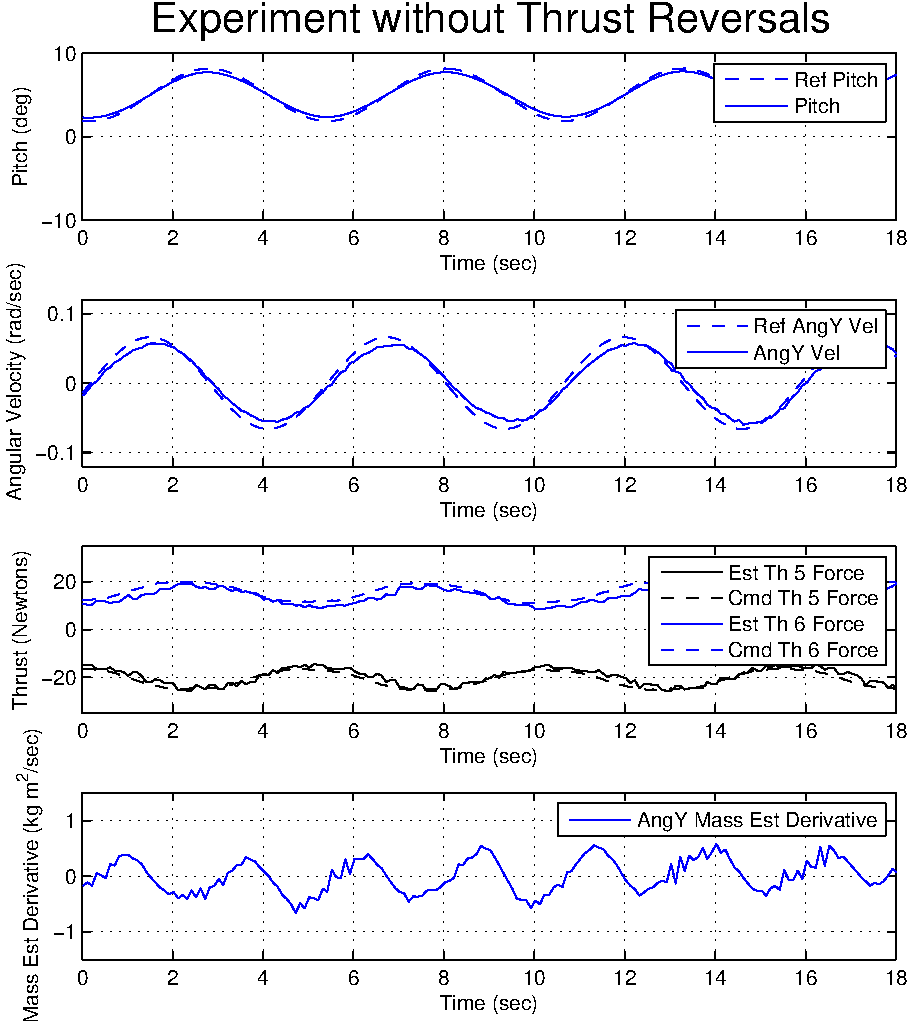
\includegraphics[width=150mm]{./chUV_AMBC/images/stictionErrorWoThrustReversals}
  \end{center}
  \caption{Eighteen seconds of data from a experiment where \ac{AMBC} was
    used to follow a single \ac{DOF} reference trajectory in pitch.
    Following the reference trajectory did not require thrust
    reversals. Thruster force was estimated using measured propeller
    angular velocity.  In the commanded/estimated thruster subplot
    thruster stiction is not observed.  The chain of events leading to a
    large negative spike in the pitch mass update law are not present
    in this experiment.}
  \label{chUV_AMBC.fig.stictionErrorWithoutThRev}
\end{figure*}
\end{center}
